\documentclass{article}

\usepackage[english]{babel}
\usepackage[utf8]{inputenc}
\usepackage{amsmath}
\usepackage{amsthm}
\usepackage{amssymb}
\usepackage{mathtools}
\usepackage{amsfonts}
\usepackage{subcaption}
\usepackage{graphicx}
\usepackage{wrapfig}
\usepackage{bbm}
\usepackage{dsfont}
\usepackage{listings}

% set up margin
\usepackage
[
  a4paper,
  left=3cm,
  right=3cm,
  top=3cm,
  bottom=3cm,
]
{geometry}

% set up header
\usepackage{fancyhdr}
\pagestyle{fancy}
\fancyhf{}
\lhead{6.438 Algorithms for Inference}
\chead{Problem Set 8}
\rhead{Hongzi Mao}
\cfoot{\thepage}
\rfoot{\footnotesize{\emph{Collaborated with: Hongzhou Ye, Zhiwei Ding}}}

% footer line
\renewcommand{\footrulewidth}{0.4pt}

% sans serif italic
\newcommand{\s}[1]{\textsf{\textit{#1}}}

% bold face sans serif
\newcommand{\bs}[1]{\textsf{\textbf{#1}}}

% set symbol
\usepackage[mathscr]{euscript}

% empty set
\let\emptyset\varnothing

% qed
\newcommand{\qeds}{\hfill\qedsymbol}

% math bold face
\newcommand{\bm}{\mathbf}

% argmax
\DeclareMathOperator*{\argmax}{argmax}
\DeclareMathOperator*{\argmin}{argmin}

% colorful reference
\usepackage{hyperref}
\usepackage{color}
\definecolor{darkred}{rgb}{0.7,0,0}
\definecolor{darkgreen}{rgb}{0,0.5,0}
\hypersetup{colorlinks=true,
        linkcolor=darkred,
        citecolor=darkgreen}
\urlstyle{same}

% independence symbol
\makeatletter
\newcommand*{\indep}{%
  \mathbin{%
    \mathpalette{\@indep}{}%
  }%
}
\newcommand*{\nindep}{%
  \mathbin{%                     % The final symbol is a binary math operator
    \mathpalette{\@indep}{\not}  % \mathpalette helps for the adaptation
                                 % of the symbol to the different math styles.
  }%
}
\newcommand*{\@indep}[2]{%
  \sbox0{$#1\perp\m@th$}%        box 0 contains \perp symbol
  \sbox2{$#1=$}%                 box 2 for the height of =
  \sbox4{$#1\vcenter{}$}%        box 4 for the height of the math axis
  \rlap{\copy0}%                 first \perp
  \dimen@=\dimexpr\ht2-\ht4-.2pt\relax
  \kern\dimen@
  {#2}
  \kern\dimen@
  \copy0 %                       second \perp
} 
\makeatother

%%%%%%%%%%%%%%%%%%%%%%%%%%%%%%%%%%%%%%%%%%%%%%%%%%%%%%%%%%%%%%%%%%%%%%%%
%%%%%%%%%%%%%%%%%%%%%%%%% Begin document here %%%%%%%%%%%%%%%%%%%%%%%%%%
%%%%%%%%%%%%%%%%%%%%%%%%%%%%%%%%%%%%%%%%%%%%%%%%%%%%%%%%%%%%%%%%%%%%%%%%
\begin{document}

\section*{Problem 8.1}
(a) Notice that the probability for observing the K samples is
\begin{align}
	P = \frac{1}{(2\pi)^{N/2}|\Sigma|^{K/2}}\exp\left\{\sum_k -\frac{1}{2}(x^{(k)}-\mu)^T\Sigma^{-1}(x^{(k)}-\mu)\right\}. \label{81a}
\end{align}

To find the Maximum Likelihood estimator for $\hat{\mu}$ and $\hat{\Sigma}$,
we notice that \eqref{81a} is jointly concave and thus take
gradient w.r.t. $\mu$ and $\Sigma$ and set them to 0. That is, we set
%
\begin{align}
\frac{\partial P}{\partial \mu} &=
%\frac{1}{(2\pi)^{N/2}|\Sigma|^{K/2}} \frac{\partial \sum_{k=1}^K\left[-{x^{(k)}}^T\Sigma^{-1}\mu-\mu^T\Sigma^{-1}x^{(k)} + \mu^T\Sigma^{-1}\mu\right]}{\partial \mu} \exp\left\{\sum_{k=1}^K -\frac{1}{2}(x^{(k)}-\mu)^T\Sigma^{-1}(x^{(k)}-\mu)\right\}
\frac{1}{(2\pi)^{N/2}|\Sigma|^{K/2}} \frac{\partial \sum_{k=1}^K\left[-\frac{1}{2}(x^{(k)}-\mu)^T\Sigma^{-1}(x^{(k)}-\mu)\right]}{\partial \mu} \exp\left\{\sum_{k=1}^K -\frac{1}{2}(x^{(k)}-\mu)^T\Sigma^{-1}(x^{(k)}-\mu)\right\} \\
&=\frac{1}{(2\pi)^{N/2}|\Sigma|^{K/2}} \left[\sum_{k=1}^K-\Sigma^{-1}(x^{(k)} - \mu)\right] \exp\left\{\sum_{k=1}^K -\frac{1}{2}(x^{(k)}-\mu)^T\Sigma^{-1}(x^{(k)}-\mu)\right\} \label{eq:81a1}\\
&= 0,
\end{align}
where in~\eqref{eq:81a1} we have used the fact that $\frac{\partial}{\partial\bm{s}}(\bm{x}-\bm{s})^T\bm{W}(\bm{x}-\bm{s}) = 2\bm{W}(\bm{x}-\bm{s})$
for symmetric matrix $\bm{W}$. Now, to set~\eqref{eq:81a1} to 0, since
$\exp(\cdot) > 0$, we have
\begin{align}
	\sum_{k=1}^K-\Sigma^{-1}(x^{(k)} - \mu) = 0.
\end{align}

This gives the MLE of $\mu$,
\begin{align}
	\hat{\mu} = \frac{1}{{K}}{\sum_{k=1}^K x^{(k)}}.
\end{align}

Similarly, we denote $E := \exp\left\{\sum_k -\frac{1}{2}(x^{(k)}-\mu)^T\Sigma^{-1}(x^{(k)}-\mu)\right\}$ and set
\begin{align}
	\frac{\partial P}{\partial \Sigma} &= 
	\frac{1}{(2\pi)^{N/2}}\frac{\partial
	\left(1/|\Sigma|^{K/2}\right)}{\partial \Sigma}E +
	\frac{1}{(2\pi)^{N/2}|\Sigma|^{K/2}}
	\frac{\partial\left\{\sum_k -\frac{1}{2}(x^{(k)}-\mu)^T
	\Sigma^{-1}(x^{(k)}-\mu)\right\}}{\partial \Sigma}E\\
	&= \frac{1}{(2\pi)^{N/2}} \frac{-K}{2}\frac{1}
	{|\Sigma|^{K/2 + 1}}\frac{\partial |\Sigma|}{\partial \Sigma}E + 
	\frac{1}{(2\pi)^{N/2}|\Sigma|^{K/2}}
	\frac{\partial\left\{\sum_k -\frac{1}{2}(x^{(k)}-\mu)^T
	\Sigma^{-1}(x^{(k)}-\mu)\right\}}{\partial \Sigma}E\\
	&=\frac{1}{(2\pi)^{N/2}} \frac{-K}{2}\frac{1}
	{|\Sigma|^{K/2 + 1}}|\Sigma|(\Sigma^{-1})^T E +
	\frac{1}{(2\pi)^{N/2}|\Sigma|^{K/2}}
    \left\{\sum_k \frac{1}{2}(\Sigma^{-1})^T (x^{(k)}-\mu)
	(x^{(k)}-\mu)^T(\Sigma^{-1})^T\right\}E \label{eq:81a2}\\
	&=0,
\end{align}
%
where in \eqref{eq:81a2} we have used the fact that $\frac{\partial\bm{a}^T\bm{X}^{-1}\bm{b}}{\bm{X}}=-(\bm{X}^{-1})^T\bm{a}\bm{b}^T(\bm{X}^{-1})^T$, and $\frac{\partial|\bm{X}|}{\partial \bm{X}} = |\bm{X}|(\bm{X}^{-1})^T$. Notice that $E>0$,
to set \eqref{eq:81a2} to 0, we have
\begin{align}
	&\frac{-K}{2}(\Sigma^{-1})^T +
    \sum_k \frac{1}{2}(\Sigma^{-1})^T (x^{(k)}-\mu)
	(x^{(k)}-\mu)^T(\Sigma^{-1})^T = 0.\\
\end{align}

This gives the MLE of $\Sigma$,
\begin{align}
	\hat{\Sigma} = \frac{1}{K}\sum_k (x^{(k)}-\hat{\mu})
	(x^{(k)}-\hat{\mu})^T.
\end{align}
\\

\noindent
(b)
\\

\noindent
(c)

\pagebreak
%%%%%%%%%%%%%%%%%%%%%%%%%%%%%%%%%%%%%%%%%%%%%%%%%%%%%%%%%%%%%%%%%%%%%%%% 
\section*{Problem 8.2}
(a) Since $p(x) \propto \exp\left(\sum_{ij}\theta_{ij} x_i x_j\right)$,
we have
\begin{align*}
p(x_i | x_{N_i}) &\propto \exp\left(\sum_{j\in N_i}\theta_{ij} x_i x_j\right).
\end{align*}
%

Normalizing the expression, we have
\begin{align}
p(x_i | x_{N_i}) &= \frac{\exp\left(\sum_{j\in N_i}\theta_{ij} x_i x_j\right)}
{\exp\left(\sum_{j\in N_i}\theta_{ij} x_j\right) +
\exp\left(-\sum_{j\in N_i}\theta_{ij} x_j\right)} \label{eq:82a_prob}
\end{align}

Thus, the expectation is
\begin{align}
	\mathbb{E}[x_i | x_{N_i}] &= \frac{
\exp\left(\sum_{j\in N_i}\theta_{ij}x_j\right) - 
\exp\left(-\sum_{j\in N_i}\theta_{ij} x_i x_j\right)}
{\exp\left(\sum_{j\in N_i}\theta_{ij} x_j\right) +
\exp\left(-\sum_{j\in N_i}\theta_{ij} x_j\right)}. \label{eq:82a_exp}
\end{align}
\\

\noindent
(b)
%
Suppose the random variable $W$ has coupling $W_1 = W_2 = \cdots = W_d$. Then for arbitrary $\beta$,
we can construct a $\beta'$ where $beta'_1 = \beta_1 + \beta_2 + \cdots + \beta_d$ and
$\beta'_2 = \beta'_3 = \cdots = \beta'_d$. Under this construction, we have
\begin{align*}
	\beta^T W &= \beta_1W_1 + \beta_2W_2 + \cdots \beta_d W_d\\
	&= \beta_1W_1 + \beta_2W_1 + \cdots \beta_d W_1 \\
	&= (\beta_1 + \beta_2 + \cdots + \beta_d)W_1 \\
	& = \beta_1' W_1 + 0W_2 + \cdots + 0W_d\\
	& = \beta'^T W.
\end{align*}
Similarly, if $\beta$ originally has $\beta_1 \neq 0$ and $\beta_2 = \beta_3 = \cdots =\beta_d = 0$, 
to make sure $\beta' \neq \beta$, we can let $\beta'_1 = \beta'_2 = \cdots = \beta'_d = \beta_1 / d$.
Then by a similar argument, we have
\begin{align*}
	\beta^T W &= \beta_1W_1 + 0W_2 + \cdots 0 W_d\\
	&= \frac{\beta_1W_1 + \beta_1W_1 + \cdots \beta_1 W_1}{d} \\
	&= \frac{\beta_1W_1 + \beta_1W_2 + \cdots \beta_1 W_d}{d} \\
	& = \frac{\beta_1}{d}W_1 + \frac{\beta_1}{d}W_2 + \cdots \frac{\beta_1}{d} W_d\\
	& = \beta'^T W.
\end{align*}
Thus, $\hat{\beta}$ is not necessarily the same as $\beta$.\qeds
\\

\noindent
(c) From the conditional probability in Equation~\eqref{eq:82a_prob}, we have
\begin{align*}
	\Pr(x_i=1|x_{N_i}) &= \frac{\exp\left(\sum_{j\in N_i}\theta_{ij} x_j\right)}
{\exp\left(\sum_{j\in N_i}\theta_{ij} x_j\right) +
\exp\left(-\sum_{j\in N_i}\theta_{ij} x_j\right)} \\
	&=
\frac{\exp\left(2\sum_{j\in N_i}\theta_{ij} x_j\right)}
{\exp\left(2\sum_{j\in N_i}\theta_{ij} x_j\right) +
1}\\
&= 
\frac{\exp\big[(2\Theta_i)^T x_{N_i}\big]}
{1 + \exp\big[(2\Theta_i)^T x_{N_i}\big]}.
\end{align*}

Now, following the logistic regression, observing the neighbor samples $x_{N_i}$ is like observing
$W$ in the problem description. Therefore, we can use algorithm A to estimate $2\Theta_i$
(corresponding to $\beta$ in the problem description) for each node $i$.
By the conclusion in (b), the challenge for this approach is that running algorithm A for different nodes
might lead to inconsistent $\hat{\Theta}$, since $\hat{\Theta}$ is not necessarily the same as the underlying
$\Theta$.
\\

\noindent
(d)
%
For arbitrary $t\in\{-1, 1\}^d$, by marginalization, we have
\begin{align*}
	\Pr(X_{N_i} = t) = \sum_{x_{k \notin N_i}}\exp\left(\sum_{mn}\theta_{mn} x_m x_n\right)
	\mathds{1}_{X_{N_i}=t}.
\end{align*}
Now we know in the above equation, $\exp\left(\sum_{mn}\theta_{mn} x_m x_n\right) > 0$ holds for all values of
$x_m$ and $x_n$. This results in $\Pr(X_{N_i} = t) > 0$. \qeds
\\

\noindent
(e)
%
By definition we have $g(X_{N_i}; 2\Theta_i) = \Pr(X_i=1|X_{N_i})$. From (c) we know that algorithm A provides
$\Pr(X_i=1|X_{N_i}) = g(X_{N_i}; 2\hat{\Theta}_i)$. This trivially leads to 
\begin{align*}
	\mathbb{E}[g(X_{N_i}; 2\Theta_i) X_j] = 	\mathbb{E}[g(X_{N_i}; 2\hat{\Theta}_i) X_j],
\end{align*}
for $\forall j \in N_i$. \qeds
\\

\noindent
(f) Starting from the result from (e) we consider
\begin{align}
	g(X_{N_i}; 2\Theta_i) = \frac{\exp\big[(2\Theta_i)^T x_{N_i}\big]}
{1 + \exp\big[(2\Theta_i)^T x_{N_i}\big]} = \frac{\exp\big[(2\hat{\Theta}_i)^T x_{N_i}\big]}
{1 + \exp\big[(2\hat{\Theta}_i)^T x_{N_i}\big]} = g(X_{N_i}; 2\hat{\Theta}_i). \label{eq:8.2f}
\end{align}
%

Notice that \eqref{eq:8.2f} indicates that
\begin{align}
	\exp\big[\Theta_i^T x_{N_i}\big] = \exp\big[\hat{\Theta}_i^T x_{N_i}\big]. \label{eq:8.2f2}
\end{align}

Now, since \eqref{eq:8.2f2} holds for any instantiation of $x_{N_i}$, consider $x_{N_i} = [-1, -1, \cdots, 1, \cdots, -1]$, where only the $k$th entry is $1$ and $-1$ elsewhere. Then we have
\begin{align*}
	&-\Theta_{i, 1} - \Theta_{i, 2} - \cdots - \Theta_{i, k-1} + \Theta_{i, k} - \Theta_{i, k+1} - \cdots \Theta_{i, |N_i|}\\
	= &-\hat{\Theta}_{i, 1} - \hat{\Theta}_{i, 2} - \cdots - \hat{\Theta}_{i, k-1} + \hat{\Theta}_{i, k} - \hat{\Theta}_{i, k+1} - \cdots \hat{\Theta}_{i, |N_i|},
\end{align*}
%
which is equivalent to
\begin{align}
	2 \Theta_{i, k} - \sum_{l=1}^{|N_i|}\Theta_{i, l} = 2 \hat{\Theta}_{i, k} - \sum_{l=1}^{|N_i|}\hat{\Theta}_{i, l}. \label{eq:82f3}
\end{align}

Now, consider taking $x_{N_i} = [1, 1, \cdots, 1]$, this leads to
\begin{align}
	\sum_{l=1}^{|N_i|}\Theta_{i, l} = \sum_{l=1}^{|N_i|}\hat{\Theta}_{i, l}. \label{eq:82f4}
\end{align}

Therefore, \eqref{eq:82f3} and \eqref{eq:82f4} result in
\begin{align}
	\Theta_{i, k} = \hat{\Theta}_{i, k}.
\end{align}

Since $k$ can be any of $\{1, 2, \cdots, |N_i|\}$. We have $\Theta_{i, k} = \hat{\Theta}_{i, k}$ holds for any coordinate, which means
\begin{align}
	\Theta_{i} = \hat{\Theta}_{i}.	
\end{align} \qeds

\pagebreak
%%%%%%%%%%%%%%%%%%%%%%%%%%%%%%%%%%%%%%%%%%%%%%%%%%%%%%%%%%%%%%%%%%%%%%%% 
\section*{Problem 8.3}
(a)
%
\begin{figure}[h!]
  \centering
  \vspace{-0.3cm}
  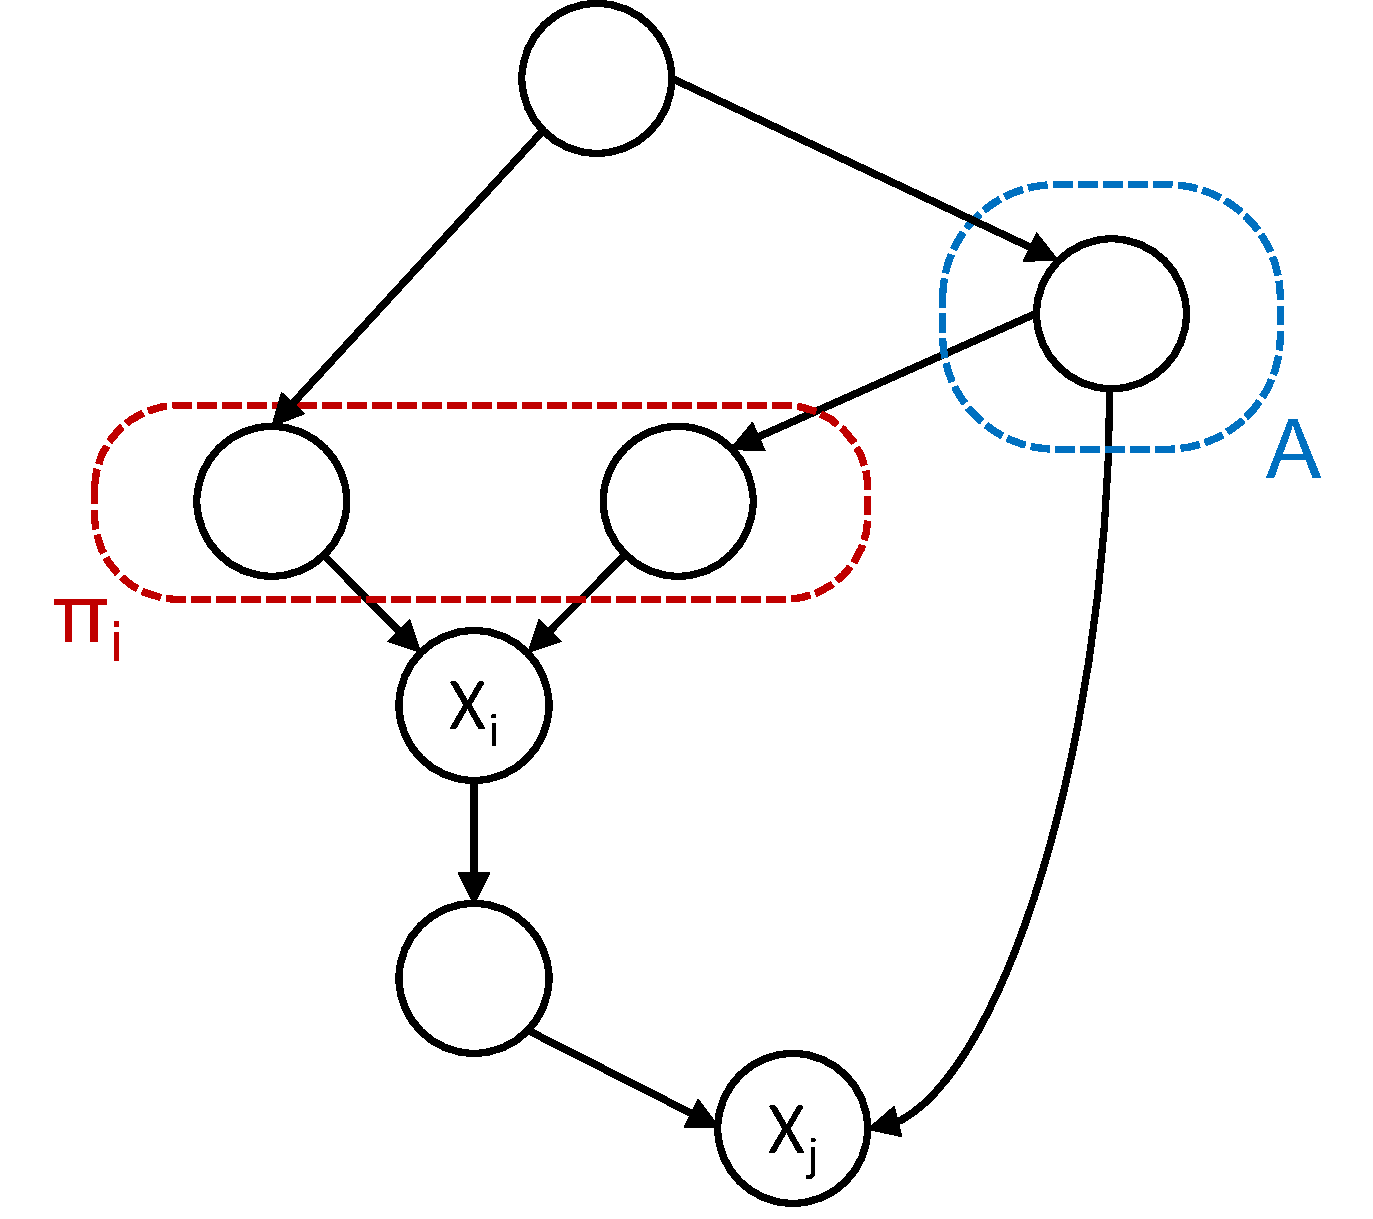
\includegraphics[width=0.35\columnwidth]{83ab.pdf}
    \vspace{-0.1cm}
  \caption{Illustration graph for 8.3.}
  \label{f:83ab}
\end{figure}
%

By construction $\pi_i$ separates all paths between $i$ and $j$. We can show this concretely by contradiction.
Suppose $X_i \nindep X_A | X_{\pi_i}$, then there exists a path between $i$ and some node in $A$ that
does not path through $\pi_i$. However, 
\begin{enumerate}
	\item such path can not be from some node in $A$ to $i$ because it has to
pass through $\pi_i$ which covers $all$ parent nodes of $i$ (e.g., the lower path from A to $i$ in
Figure~\ref{f:83ab});
	\item such path can not have both some node in $A$ and $i$ both as descendent, because again
this path has to path through $\pi_i$ (e.g., top path from $A$ to $i$ in Figure~\ref{f:83ab});
	\item also, such path can not originate from $i$ and lead to $A$,
because by construction no node in A is a descendant of $i$;
	\item finally,
there is no path that goes into $\pi_i$ from both $i$ and $A$ (the head to head condition),
because $\pi_i$ is parent set and this would lead to a loop.
\end{enumerate}
Therefore, we have $X_i \indep X_A | X_{\pi_i}$.
\qeds
\\

\noindent
(b) We show this by contradiction.
Suppose $X_j \nindep X_{\pi_i} | X_{i}, X_A$, then there exists a path between $\pi_i$ and $j$ that
does not path through $i$ or any node in $X_A$. However, 
\begin{enumerate}
	\item such path can not be from some node in $\pi_i$ to $j$ because it has to
pass through $i$ since $\pi_i$ contains $all$ parent nodes of $i$ (e.g., any path from $\pi_i$ to $j$ in
Figure~\ref{f:83ab});
	\item such path can not have both some node in $\pi_i$ and $j$ both as descendent, because such 
will also have both $i$ and $j$ both as descendent and 
by construction all backdoor paths have to pass through $A$ (e.g., the rightmost path in Figure~\ref{f:83ab});
	\item also, such path can not originate from $j$ and lead to $\pi_i$,
because $j$ is descendant of $i$ and this leads to illegal cycle;
	\item finally,
there is no path that goes into $\pi_i$ or $A$ that is from both $i$ and $j$ (the head to head condition),
because $\pi_i$ and $A$ are ancestors of $i$ and path into them lead to cycle.
\end{enumerate}
Therefore, we have $X_j \indep X_{\pi_i} | X_{i}, X_A$.
\qeds
\\

\noindent
(c)  We first notice that the parent set is an adjustment set. That is
\begin{align*}
	P_{X_j|do(X_i = x_i)}(x_j) = \sum_{x_{\pi_i}}P_{X_{\pi_i}}(x_{\pi_i})P_{X_{j}|X_i, X_{\pi_i}}(x_j|x_i, x_{\pi_i}).
\end{align*}
\\

Now we notice that
\begin{align*}
	&\;\;\;\;\sum_{x_{\pi_i}}P_{X_{\pi_i}}(x_{\pi_i})P_{X_{j}|X_i, X_{\pi_i}}(x_j|x_i, x_{\pi_i}) \\
	&=
	\sum_{x_{\pi_i}}P_{X_{\pi_i}}(x_{\pi_i})\frac{P_{X_{j}, X_i, X_{\pi_i}}(x_j, x_i, x_{\pi_i})}
	{P_{X_i, X_{\pi_i}}(x_i, x_{\pi_i})} \\
	&= \sum_{x_{\pi_i}}P_{X_{\pi_i}}(x_{\pi_i})\frac{\sum_{x_A}P_{X_{j}, X_i, X_{\pi_i}, X_A}(x_j, x_i, x_{\pi_i}, x_A)}
	{P_{X_i, X_{\pi_i}}(x_i, x_{\pi_i})} \\
	&= \sum_{x_{\pi_i}}P_{X_{\pi_i}}(x_{\pi_i})\frac{\sum_{x_A}P_{X_{j}, X_i, X_{\pi_i}, X_A}(x_j, x_i, x_{\pi_i}, x_A)}
	{P_{X_i, X_{\pi_i}, X_A}(x_i, x_{\pi_i}, x_A)}
	\frac{P_{X_i, X_{\pi_i}, X_A}(x_i, x_{\pi_i}, x_A)}
	{P_{X_i, X_{\pi_i}}(x_i, x_{\pi_i})}\\
	&=\sum_{x_A}\sum_{x_{\pi_i}}P_{X_{\pi_i}}(x_{\pi_i})P_{X_{j}|X_i, X_{\pi_i}, X_A}(x_j|x_i, x_{\pi_i}, x_A)
	P_{X_A|X_i, X_{\pi_i}}(x_A|x_i, x_{\pi_i})\\
	&= \sum_{x_A}\sum_{x_{\pi_i}}P_{X_{\pi_i}}(x_{\pi_i})P_{X_{j}|X_i, X_A}(x_j|x_i, x_A)
	P_{X_A|X_i, X_{\pi_i}}(x_A|x_i, x_{\pi_i}) \quad (\text{since }X_j \indep X_{\pi_i} | X_{i}, X_A)\\
	&= \sum_{x_A}\sum_{x_{\pi_i}}P_{X_{\pi_i}}(x_{\pi_i})P_{X_{j}|X_i, X_A}(x_j|x_i, x_A)
	P_{X_A|X_{\pi_i}}(x_A|x_{\pi_i}) \quad (\text{since }X_i \indep X_A | X_{\pi_i})\\
	&= \sum_{x_A}\sum_{x_{\pi_i}}P_{X_{j}|X_i, X_A}(x_j|x_i, x_A)
	P_{X_A, X_{\pi_i}}(x_A, x_{\pi_i}) \\
	&= \sum_{x_A}P_{X_{j}|X_i, X_A}(x_j|x_i, x_A)
	\sum_{x_{\pi_i}}P_{X_A, X_{\pi_i}}(x_A, x_{\pi_i})\\
	&= \sum_{x_A}P_{X_A}(x_A)P_{X_{j}|X_i, X_A}(x_j|x_i, x_A).
\end{align*}

Thus, we reach $P_{X_j|do(X_i = x_i)}(x_j) = \sum_{x_A}P_{X_A}(x_A)P_{X_{j}|X_i, X_A}(x_j|x_i, x_A)$ and
$X_A$ is a valid adjustment set for $X_i$ and $X_j$. \qeds
\\
\\
\\

\noindent
(d) By the definition of backdoor criterion, $\{X_6\}$ satisfies the condition.

\pagebreak
%%%%%%%%%%%%%%%%%%%%%%%%%%%%%%%%%%%%%%%%%%%%%%%%%%%%%%%%%%%%%%%%%%%%%%%% 
\section*{Problem 8.4}
(a) The causal DAG is shown in Figure~\ref{f:84a}.
%
\begin{figure}[h!]
  \centering
  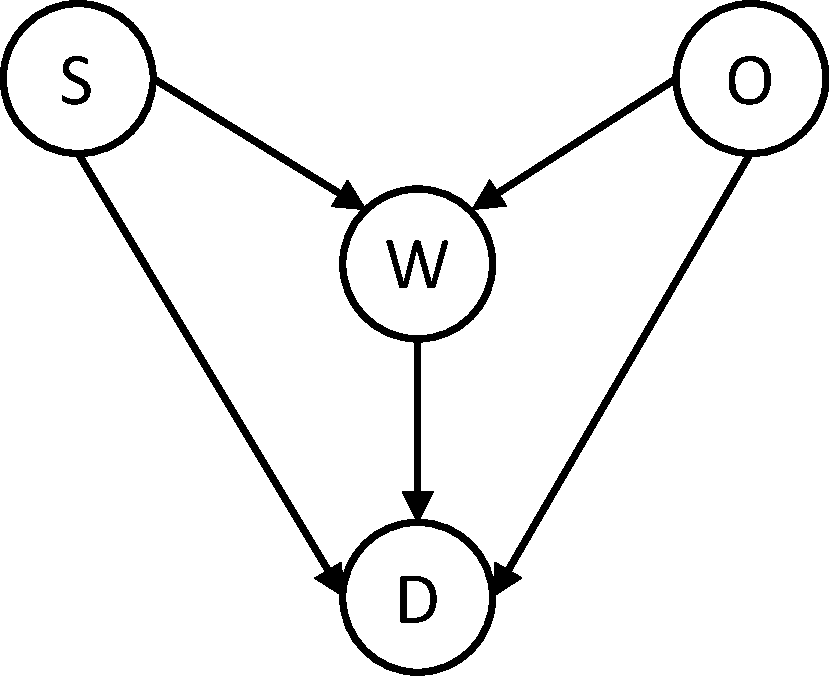
\includegraphics[width=0.3\columnwidth]{84a.pdf}
    \vspace{-0.1cm}
  \caption{Casual DAG for 8.4(a).}
  \label{f:84a}
\end{figure}
\\

\noindent
(b) (i) True. This is because
\begin{align*}
	P_{W|do(S=s)} 
	&= \mathds{1}_{S=s} \sum_{S, D, O} p(O)p(W|S,O)p(D|S,O, W)\\
	&= \mathds{1}_{S=s} \sum_{S, O} p(O)p(W|S,O) \sum_D p(D|S,O, W) \\
	&= \sum_{O} p(O)p(W|s,O) \\
	&= \sum_{O} p(O)\frac{p(W, s, O)}{p(s, O)} \\
	&= \sum_{O} p(O)\frac{p(W, s, O)}{p(s)p(O)}\\
	&= \frac{\sum_{O}p(W, s, O)}{p(s)} \\
	&= \frac{p(W,s)}{p(s)}\\
	&=p(W|s).
\end{align*} \qeds
\\
%

\noindent
(ii) True. This is because
\begin{align*}
	P_{D|do(S=s)} 
	&= \mathds{1}_{S=s} \sum_{S, W, O} p(O)p(W|S,O)p(D|S,O, W)\\
	&= \mathds{1}_{S=s} \sum_{S, W, O} p(O)p(D, W|S,O)  \\
	&= \mathds{1}_{S=s} \sum_{S, O}p(O) \sum_W  p(D, W|S,O)  \\
	&= \sum_{O} p(O)p(D|s,O) \\
	&= \sum_{O} p(O)\frac{p(D, s, O)}{p(s, O)} \\
	&= \sum_{O} p(O)\frac{p(D, s, O)}{p(s)p(O)}\\
	&= \frac{\sum_{O}p(D, s, O)}{p(s)} \\
	&= \frac{p(D,s)}{p(s)}\\
	&=p(D|s).
\end{align*}\qeds
\\
%

\noindent
(iii) False. This is apparent because $S \rightarrow W \leftarrow O$ forms the head-to-head V-structure in
directed graphical model. Thus, condition on the observation of $W$ makes $S$ and $O$ dependent on each other.\qeds
\\
\\

\noindent
(c)

(i) $P_{D|do(S=1)}(1) > P_D(1)$.
\\

(ii) $P_{W|do(S=1)}(l) > P_W(l)$. (Parsing the sentence differently, one can think of the ``increase'' means increasing from to the group that is controlled not to smoke. In that case, the probability statement is
$P_{W|do(S=1)}(l) > P_{W|do(S=0)}(l)$.)
\\

(iii) $P_{D|W}(1|l) > P_D(1)$. (Parsing the sentence differently, one can think of the ``higher'' means higher than the group with high birth weight. In that case, the probability statement is
$P_{D|W}(1|l) > P_{D|W}(1|h)$.)
\\

(iv) $P_{D|W, S}(1|l, 1) < P_{D|W, S}(1|l, 0)$.

\end{document}